	\documentclass{article}
			
		\usepackage{parskip}
		\usepackage{listings}
		\usepackage{xcolor}
		\usepackage{textcomp}
			
		%STYLE AND COLOR DEFINITION FOR SOURCE CODE 	
		\newcommand{\PHPamountofcolor}{75}
		\newcommand{\SourceCodeContext}{5}
		%Lets define the php language colors:
		\definecolor{PHP_comment_old}{HTML}{FF8000}
		\colorlet{PHP_comment}{PHP_comment_old!\PHPamountofcolor!black}
		\definecolor{PHP_default_old}{HTML}{000000}
		\colorlet{PHP_default}{PHP_default_old!\PHPamountofcolor!black}
		\definecolor{PHP_keyword_old}{HTML}{6c9c11}
		\colorlet{PHP_keyword}{PHP_keyword_old!\PHPamountofcolor!black}
		\definecolor{PHP_emph1_old}{HTML}{0F58A2}
		\colorlet{PHP_emph1}{PHP_emph1_old!\PHPamountofcolor!black}
		\definecolor{PHP_emph2_old}{HTML}{CCAA00}
		\colorlet{PHP_emph2}{PHP_emph2_old!\PHPamountofcolor!black}
		\definecolor{PHP_emph4_old}{HTML}{C60484}
		\colorlet{PHP_emph4}{PHP_emph4_old!\PHPamountofcolor!black}
		\definecolor{PHP_string_old}{HTML}{C78F0A}
		\colorlet{PHP_string}{PHP_string_old!\PHPamountofcolor!black}
		\definecolor{PHP_variable_old}{HTML}{C82210}%C82210
		\colorlet{PHP_variable}{PHP_variable_old!\PHPamountofcolor!black}
		\definecolor{PHP_number_old}{HTML}{BF1CA6}
		\colorlet{PHP_number}{PHP_number_old!\PHPamountofcolor!black}
		%Now we want to highlight the variables. This will be done by triggering the function \PHPhighlightvar at the start of any $ run. This function wil only highlight variables and any other identifiers will be ignored. Luckily lstlisting will only give correct identifiers so we only will have to check if the previous call was made with a $
		\usepackage{fontspec}
		\setmonofont{Courier}
		%\usepackage[utf8]{inputenc}
		%\usepackage[T1]{fontenc}
		%\usepackage{courier, textcomp}
		\usepackage{etoolbox}
		\newtoggle{InString}{}% Keep track of if we are within a string
		\togglefalse{InString}% Assume not initally in string
		
		\newcommand*{\ColorIfNotInString}[1]{\iftoggle{InString}{#1}{\color{PHP_number}#1}}%

		%helper
		
		\newcommand{\PHPhighlightvar}[1]{\ifnum\theDollarFlag=1 \color{PHP_variable} \fi#1\setcounter{DollarFlag}{0}}
		\newcounter{DollarFlag}
		
		%images
		\usepackage{graphicx}
		\graphicspath{ {images/} }
		\usepackage{wrapfig}
		\usepackage{subcaption}
		
		
			
			
			
		
			
			\title{Machine Learning: Sixth Home Work \\ \bigskip \large Bayesian Networks}

			\author{Edoardo Ghini}
			
			\begin{document}
			
			\textbf{\maketitle}
			\pagenumbering{gobble}
			
			\bigskip\bigskip\bigskip
			\begin{center}
			
\includegraphics[width=0.5\textwidth]{laSapienza}
			\end{center}
			\bigskip\bigskip\bigskip
			\textbf{
			Dipartimento di Ingegneria dell'Università di Roma La Sapienza}
			

			\newpage
			\pagenumbering{roman}
			\tableofcontents
			\newpage
			\pagenumbering{arabic}
			
			
			
			
			
			%SETTING STYLE OF SOURCE CODE
			\lstset{
		  language        = php,
		  basicstyle      = \footnotesize\ttfamily,
		  keywordstyle    = \color{PHP_keyword},
		  stringstyle     = \color{PHP_string!90!black}\toggletrue{InString},
		  %this allows highlighting of variables:
		  literate        =  {\$}{{\iftoggle{InString}{\$}{\setcounter{DollarFlag}{1}\color{PHP_variable}\$\color{PHP_default}}}}1
		%    {"}{{{\ProcessQuote{"}}}}1% Disable coloring within double quotes
		%    {'}{{{\ProcessQuote{'}}}}1% Disable coloring within single quote
		    {0}{{{\ColorIfNotInString{0}}}}1
		    {1}{{{\ColorIfNotInString{1}}}}1
		    {2}{{{\ColorIfNotInString{2}}}}1
		    {3}{{{\ColorIfNotInString{3}}}}1
		    {4}{{{\ColorIfNotInString{4}}}}1
		    {5}{{{\ColorIfNotInString{5}}}}1
		    {6}{{{\ColorIfNotInString{6}}}}1
		    {7}{{{\ColorIfNotInString{7}}}}1
		    {8}{{{\ColorIfNotInString{8}}}}1
		    {9}{{{\ColorIfNotInString{9}}}}1,
		  identifierstyle = \color{PHP_default}\PHPhighlightvar,
		  commentstyle    = \color{PHP_comment}\slshape,
		  emph            =[1]{require_once, require, include_once, include, namespace, use, class, function, new},
		  emphstyle       =[1]\color{PHP_emph1},%\bf,
		  emph            =[2]{echo, empty, isset, array, instanceof},
		  emphstyle       =[2]\color{PHP_emph2},%\bf,
		  emph            =[3]{var, const, abstract, 
		                        protected, private, public,
		                        static, final, extends, implements,
		                        global, if, else, foreach ,for,
		                        endforeach, endif, endfor, elseif,
		                        as},
		  emphstyle       =[3]\color{PHP_keyword},%\bf,
		  emph            =[4]{return, throw, exit, __halt_compiler, continue, break},
		  emphstyle       =[4]\color{PHP_emph4},%\bf,
		  breaklines      = true,
		  captionpos      = b,
		  rulecolor       =\color{black},
		  keywords    ={__halt_compiler,    abstract,   and,    array,
		                    as, break,  callable,   case,   catch,  class,
		                    clone,  const,  continue,   declare,    default,
		                    die,    do, echo,   else,   elseif,
		                    empty,  enddeclare, endfor, endforeach, endif,
		                    endswitch,  endwhile,   eval,   exit,   extends,
		                    final,  finally,    for,    foreach,    function,
		                    global, goto, if,   implements, include,
		                    include_once,   instanceof, insteadof,
		                    interface,  isset, list,    namespace,
		                    new,    or, print, private, protected,  public,
		                    require,    require_once, return,   static,
		                    switch, throw,  trait, try, unset, use, var,
		                    while,  xor,    yield,
		  },
		  numbers=left,
		  stepnumber=1,  
		  numberfirstline=true,
		  numberstyle=\footnotesize,
		  xleftmargin=4.0ex,
		  upquote=true,
		  showlines=true
		  }	
			
			\renewcommand{\lstlistingname}{Code}

			
			\part{Introduction}
			
				\section{Scope}
I was supposed to familiarise with bayesian networks used in stochastic modelling. 
				\section{Objectives}
				Learning to model graph-like networks with a Bayesian approach for three different cases.

\newpage
			\part{Development}
				\section{First case}
\begin{center}	
\begin{figure}
\centering
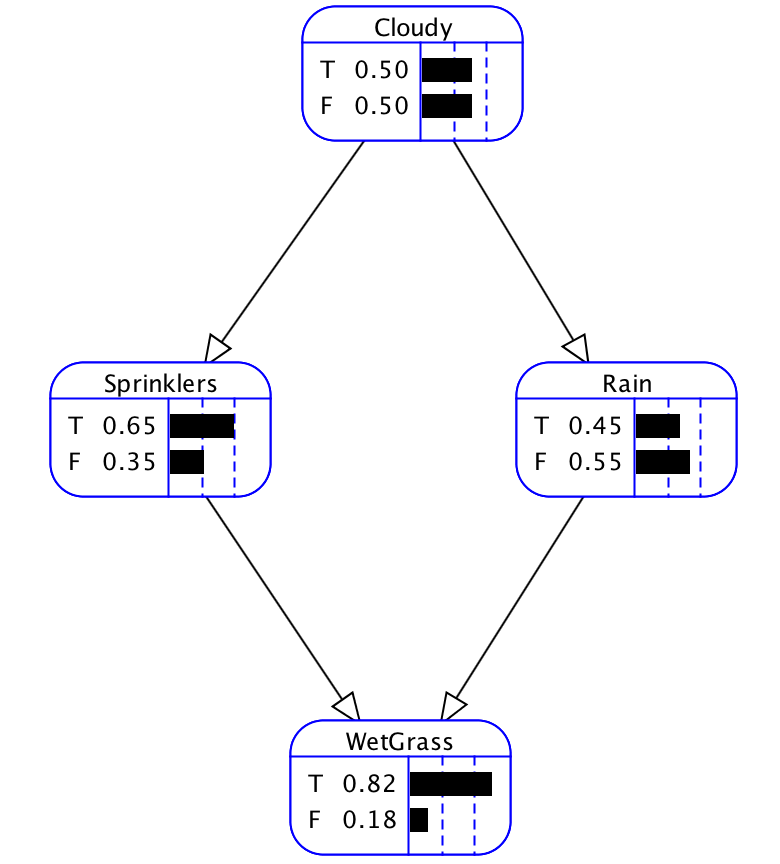
\includegraphics[width=0.9\textwidth]{fig1}
\caption{}
\label{fig:1}
\end{figure}
\end{center}

I have built a model that represents the conditional bounds between stochastic atoms.
In particular, in fig(1), there is the graphical model that corresponds to the following joint probability distribution: 
\medskip
P( Cloudy, Sprinklers, Rain,WetGrass) = P( Cloudy ) P( Sprinklers| Cloudy) P( Rain| Cloudy) P( WetGrass| Sprinklers, Rain)
\smallskip
In fig(2) there is also the result, according to the conditional probability, after that two observations have been made.

\begin{center}	
\begin{figure}
\centering
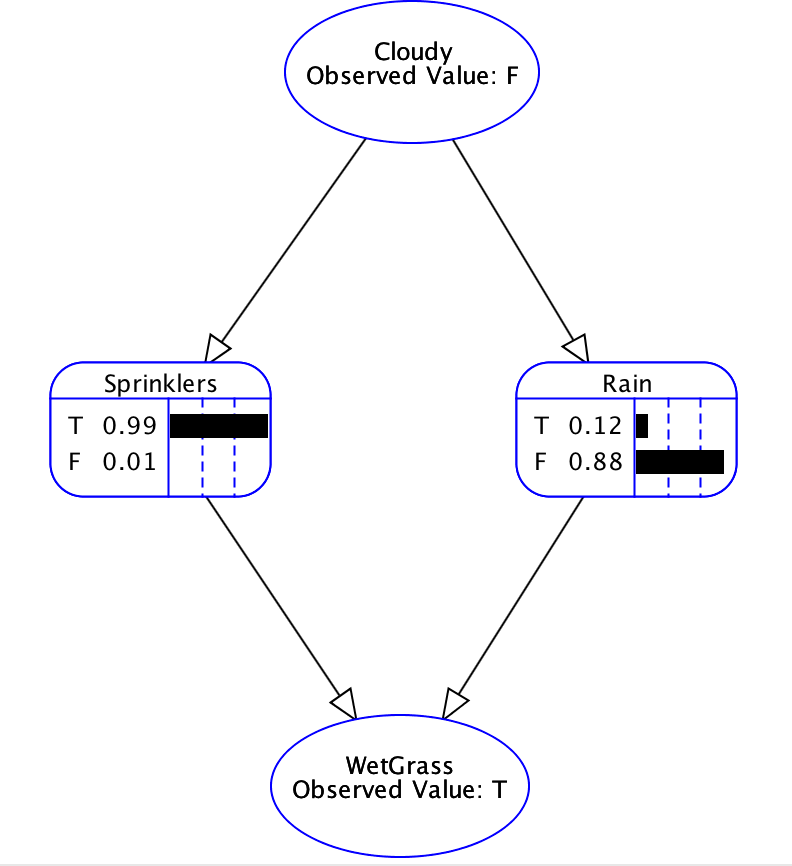
\includegraphics[width=0.9\textwidth]{fig2}
\caption{}
\label{fig:2}
\end{figure}
\end{center}

				\section{Second case}
				Then I build a model in order to reconstruct the probability distribution of a random coin extraction between three differently weighted coins in terms of probabilities between head and tail outcomes.
				In fig(3), given a prior knowledge on three trows made with a unique coin, there is the guess of the bayesian network on which coin has been extracted. 
\begin{center}
\begin{figure}
\centering
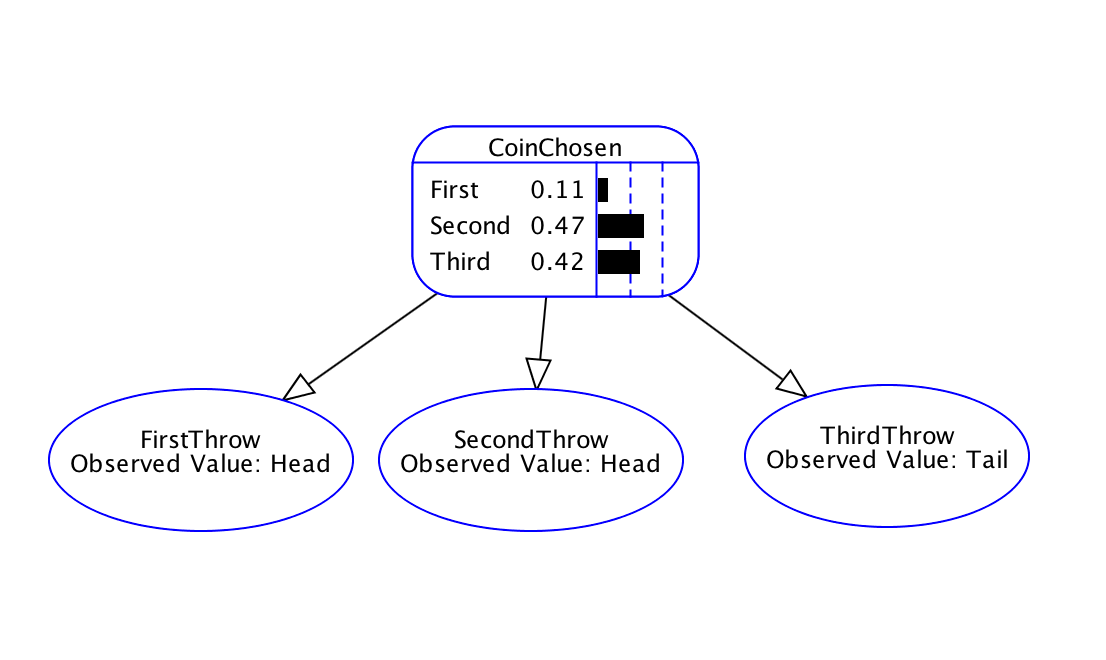
\includegraphics[width=0.9\textwidth]{fig3}
\caption{}
\label{fig:3}
\end{figure}
\end{center}


				\section{Third case}
Finally, the last assignment consisted of a modification of an already finished model that describes probabilities of events after that a fire alarm goes on.
Essentially, I added a branch to the graph linking two nodes: the former was the node which symbolises  that the alarm has gone off, the latter was a new node which represents the probability that someone could call their mother.
Accordingly, in fig(4), there is the modified bayesian network corresponding to the joint probabilty distribution written above: 
\medskip
P( tampering, fire, alarm, smoke, leaving, report)=
\smallskip 
	P( tampering)* P( fire)* P(alarm| tampering,fire)* P(smoke| fire)* P(leaving| alarm)* P(report| leaving)

\begin{center}
\begin{figure}
\centering  
        \begin{subfigure}[b]{0.48\textwidth}
                \centering
                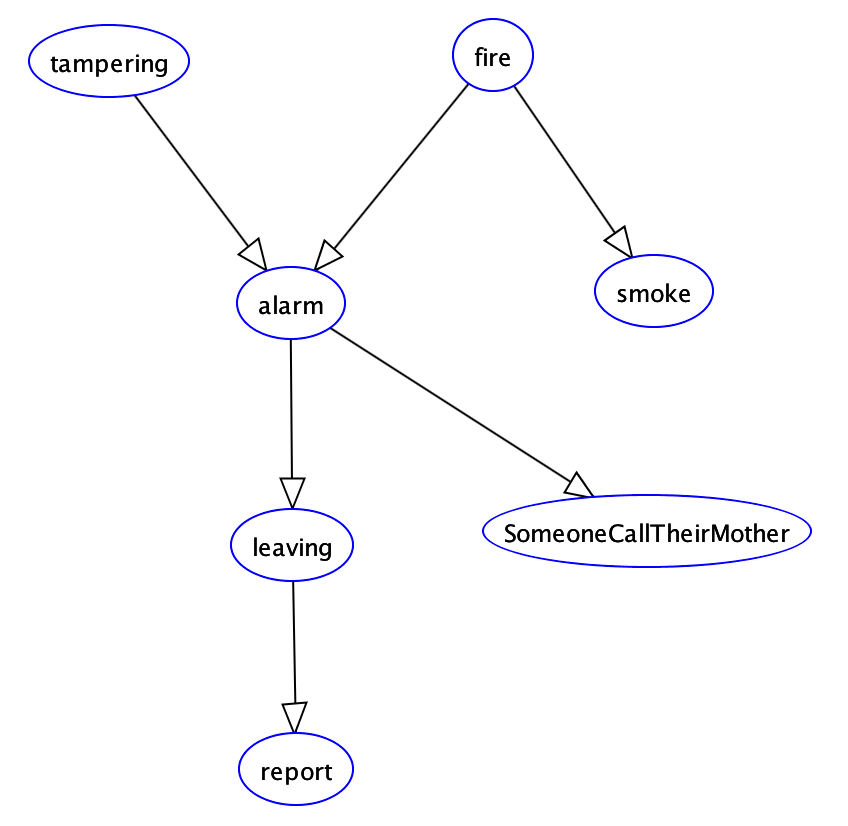
\includegraphics[width=\linewidth]{fig4}
        \end{subfigure}\hfill
        \begin{subfigure}[b]{0.48\textwidth}
                \centering
                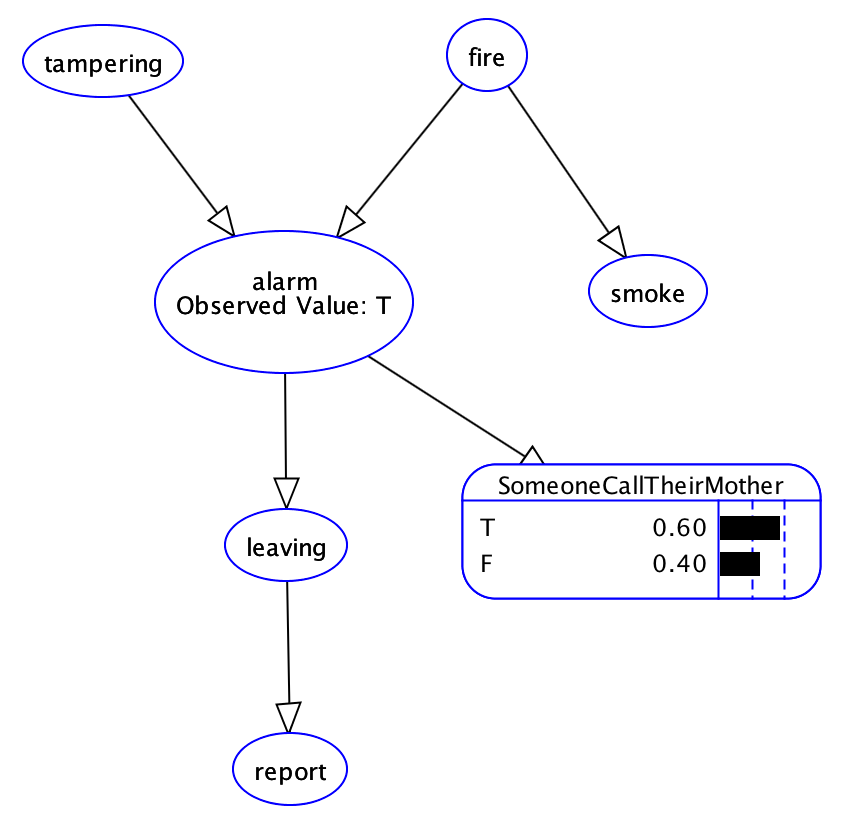
\includegraphics[width=\linewidth]{fig5}
        \end{subfigure}
        \label{fig:4}
\end{figure}
\end{center}		


	
\newpage
			\part{Conclusions}
				
In the final analysis bayesian network approach could be extremely powerful in order to visualise and understand the stochastic representation of complex scenarios. On the other hand, when there would be plenty of conditional dependencies among the nodes, it become a disorienting representation 

			
		\end{document}
